\chapter{Projet Find Your Teams}

\section{Introduction}

Le second projet est aussi guidé par le chercheur, mais avec une approche complètement différente.
C’est une approche « Startups » où nous avons cherché un domaine que nous apprécions et nous avons essayé de résoudre un problème existant dans ce domaine.
Pour ce projet, nous avons choisi un domaine que nous aimons : le sport.
Nous n'avions jamais entendu parler d'un réseau social permettant de trouver un partenaire ou un club pour s'entraîner dans n'importe quel sport.
Après quelques recherches, nous avons constaté qu'il n'existait pas encore une telle application sur le marché.
Ce projet a pour principal objectif de renforcer et d'augmenter les compétences déjà acquises sur le projet Bac à Sable.

\section{Technologies utilisées}

\begin{multicols}{2}
    \begin{itemize}
        \item Angular : Un framework JavaScript qui facilite la création d'applications Web interactives.
        \item Node.js : Un environnement d'exécution JavaScript côté serveur.
        \item TypeScript : Un langage de programmation qui est une extension de JavaScript.
        \item Go : Un langage de programmation simple et performant.
        \item MongoDB : Une base de données utilisée dans les applications Web.
        \item GitHub Actions : Un service pour automatiser diverses tâches telle que le déploiement.
        \item GitHub : Une plateforme de développement collaborative basée sur Git.
        \item Google Cloud Platform : Une suite de services cloud proposée par Google.
        \item Terraform : Un outil d'infrastructure en tant que code (IaC).
        \item Google Cloud Run : Un service qui permet d'exécuter des conteneurs Docker.
        \item Google Cloud Build : Un service qui permet d'automatiser la construction d’applications.
        \item Google Cloud Artifact Registry : Un service qui permet de stocker des images de conteneurs.
        \item Google Cloud Secret Manager : Un service de gestion des secrets.
        \item Google Cloud DNS : Un service pour gérer et résoudre les noms de domaine.
    \end{itemize}
\end{multicols}

\section{Objectif du projet}

L’approche startup signifie qu’avant de commencer la partie de développement, il faut analyser ce qui existe, ce qui a fonctionné et ce qui fonctionne à l’heure actuelle. Il faut également analyser le marché, définir les objectifs de l’application, son design, sa maquette et ensuite développer. L’objectif de l’application est de permettre à un utilisateur de créer un événement sportif, d'afficher une carte des événements et d'avoir un canal de message.

\section{Conception}

\subsection{Première conception de l’application}

Pour la première partie du développement, le chercheur m’a laissé développer à ma manière afin de voir ma gestion de projet individuel.
J’ai voulu réaliser tous les éléments souhaités dans l’application et y rajouter des idées que j’avais sur le moment.
Très vite, j’avais plein d’idées mais pas encore très concrètes, et j’étais un peu perdu. Le chercheur m’a donc expliqué qu’il fallait avoir une approche minimaliste pour déployer au plus vite, en se concentrant sur les fonctionnalités minimales de l’application. Nous avons utilisé une méthode de « refactoring » pour rendre le code réutilisable et minimaliste.

\subsection{Développement des fonctionnalités nécessaires}

Je me suis concentré sur le développement des fonctionnalités nécessaires au fonctionnement de l’application :
\begin{itemize}
    \item Une carte interactive listant chaque événement.
    \begin{figure}[H]
        \centering
        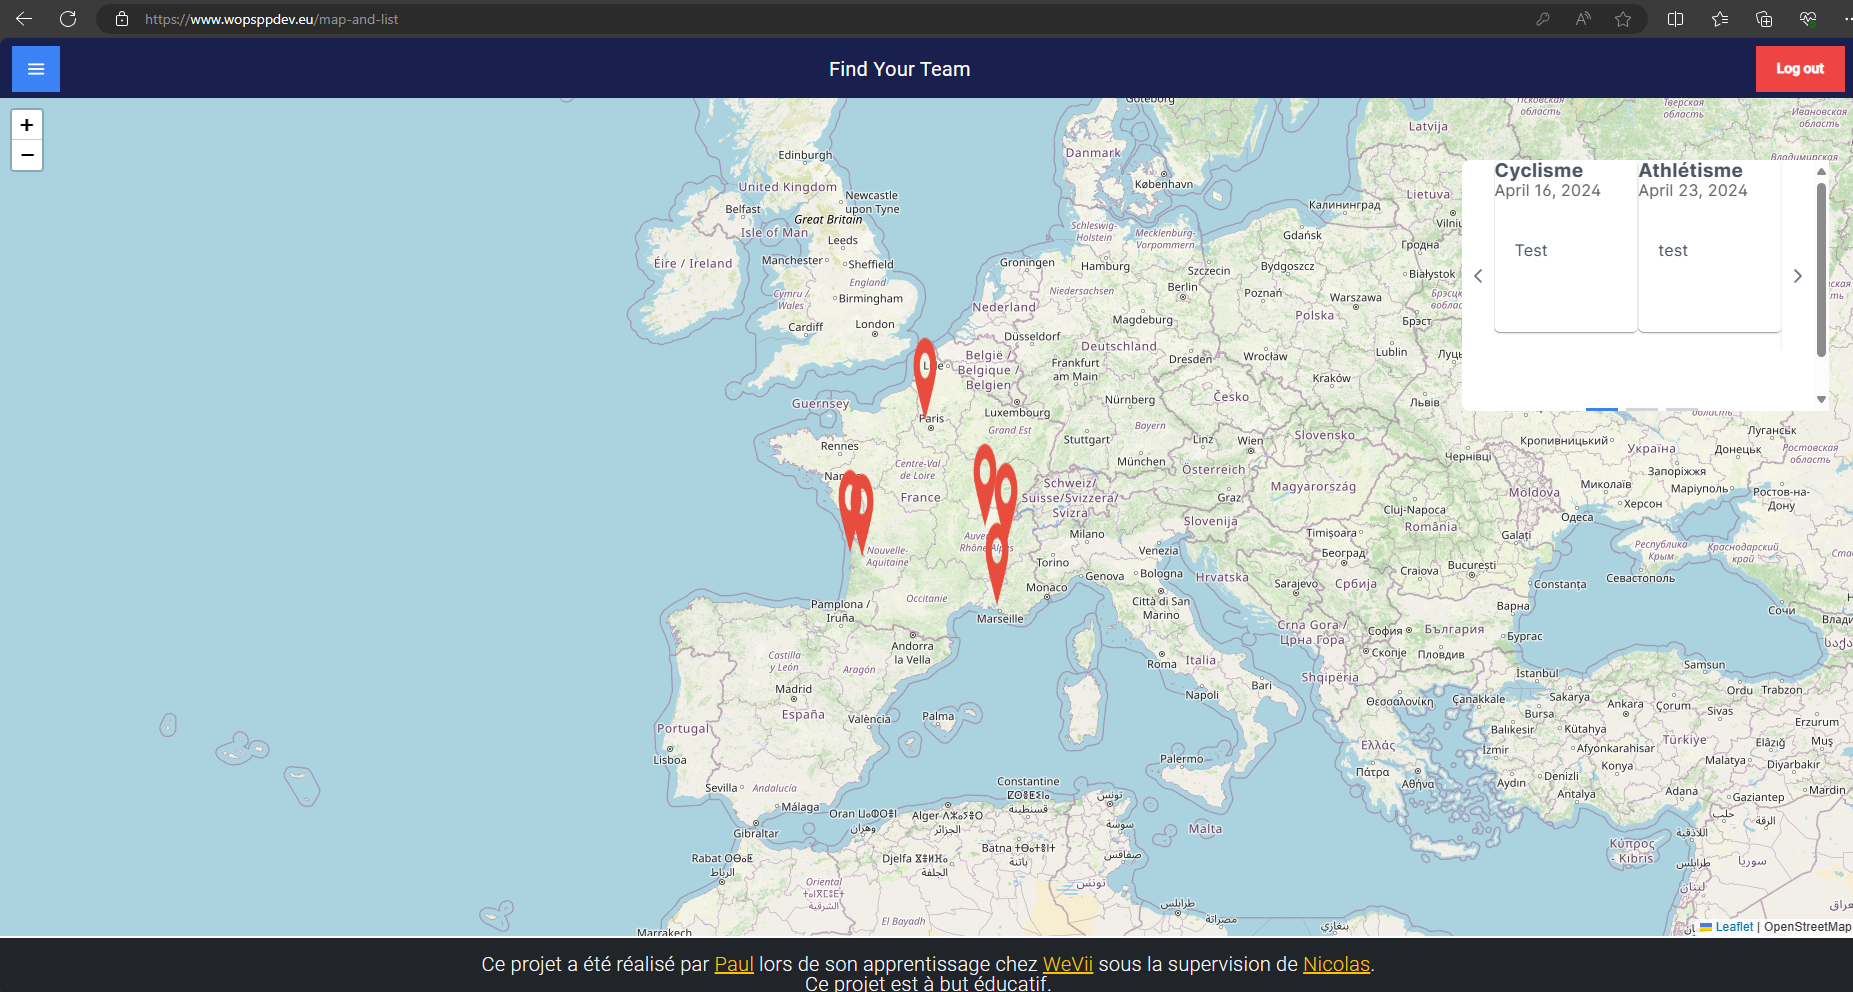
\includegraphics[width=0.45\textwidth]{image/fytMap}
        \caption{Carte interactive des évènements}
        \label{fig:fytMap}
    \end{figure}
    \item Un formulaire permettant d’ajouter un événement.
    \begin{figure}[H]
        \centering
        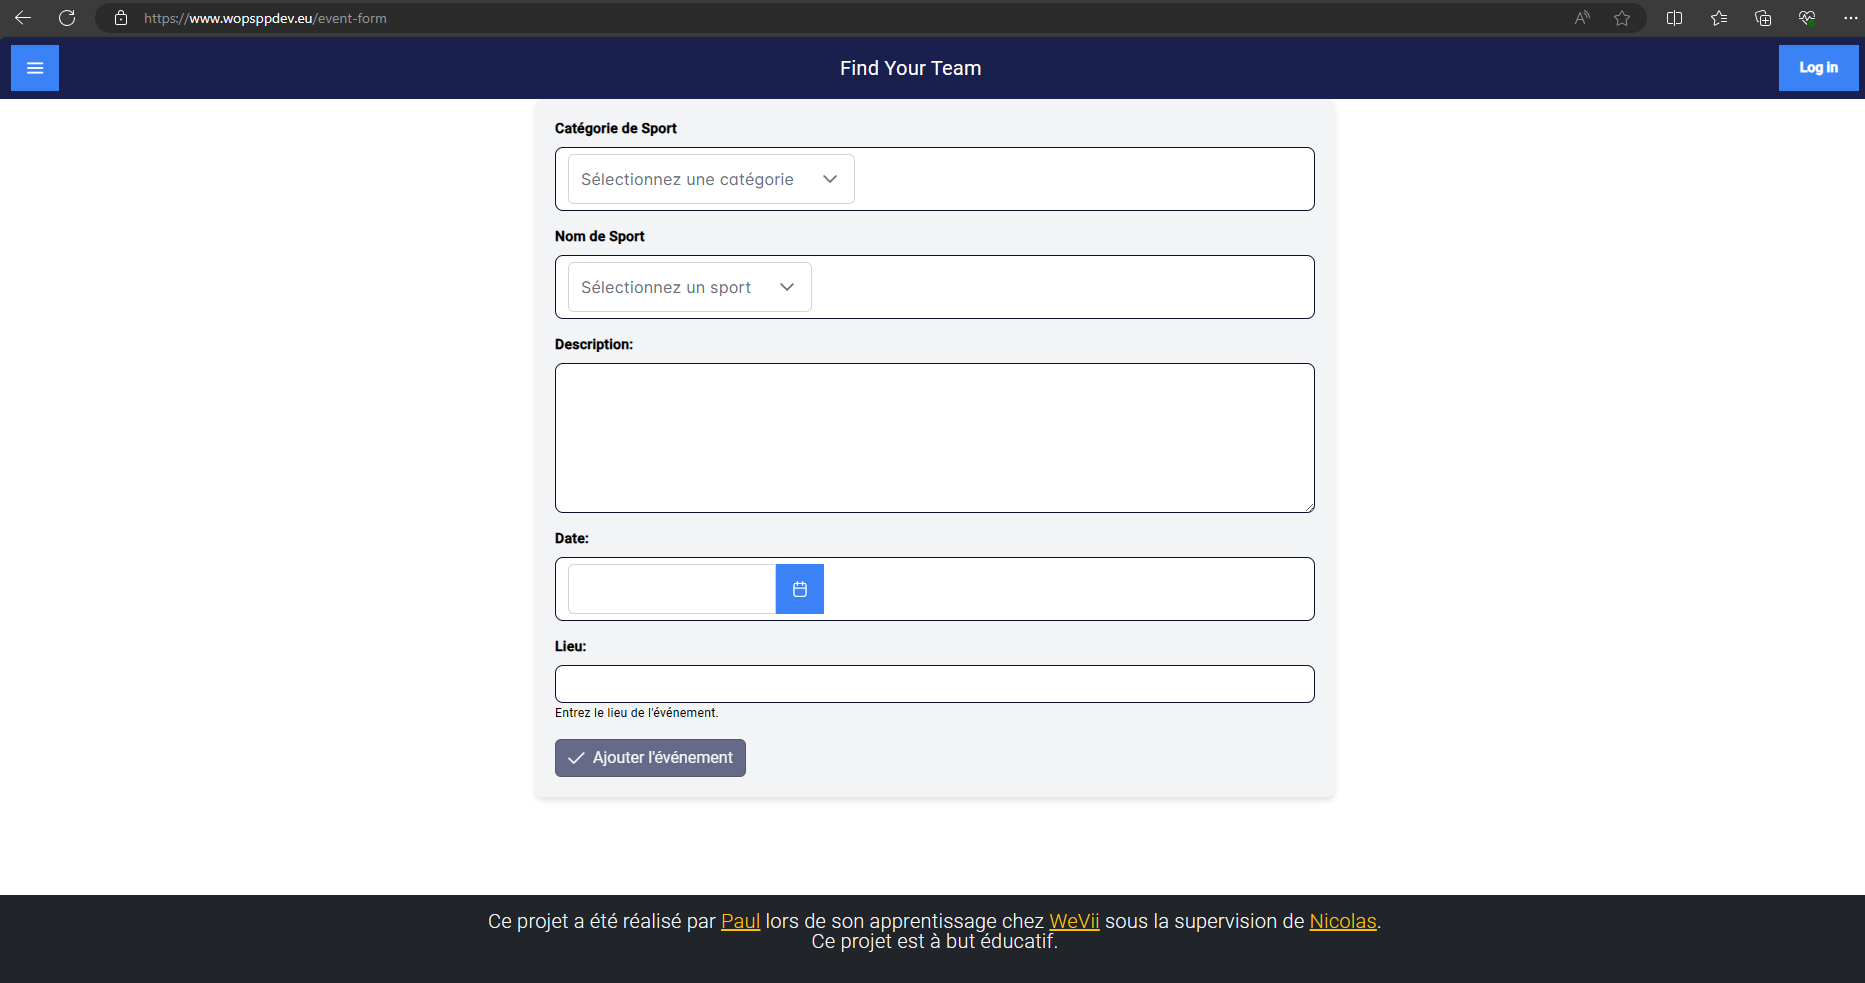
\includegraphics[width=0.45\textwidth]{image/fytForm}
        \caption{Formulaire d'ajout d'événement}
        \label{fig:fytForm}
    \end{figure}
    \item Une liste des évènements permettant au créateur de l’événement de modifier ou supprimer l’événement.
\end{itemize}

Une fois l’application développée de manière minimaliste, j'ai créé une instance de machine virtuelle (VM), un nom de domaine et conteneurisé mon application.
Commencer à déployer sur une VM permet de faire du diagnostic réseau et d’avoir la main sur tout en cas de problème.
Une fois le déploiement réussi, il faut mettre en place un déploiement continu pour automatiser ce processus, car le déploiement est une tâche répétitive.
Pour cela, j’ai choisi GitHub Actions qui permet de faire un déploiement directement avec SSH et d'y mettre ses instructions.

\section{Amélioration de l’application}

J'ai recueilli les retours des utilisateurs extérieurs au projet pour connaître leurs avis sur l’application.
Voici un exemple de retour reçu :
\begin{figure}[H]
    \centering
    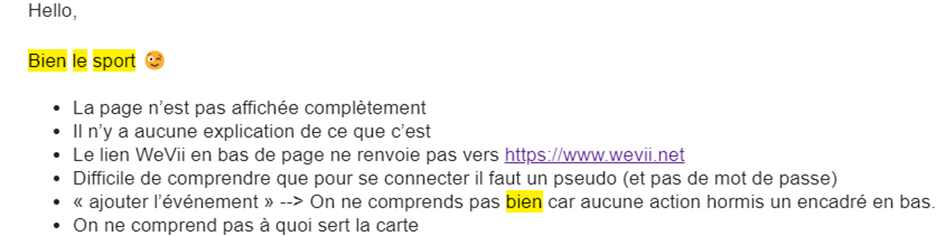
\includegraphics[width=\textwidth]{image/bienLeSportFYT}
    \caption{Commentaire sur l'application}
    \label{fig:commentaire_application}
\end{figure}

Les utilisateurs avaient du mal à comprendre l'application, j'ai donc ajouté une page d'accueil pour mieux expliquer son fonctionnement.
\begin{figure}[ht]
    \centering
    \begin{minipage}{.45\textwidth}
        \centering
        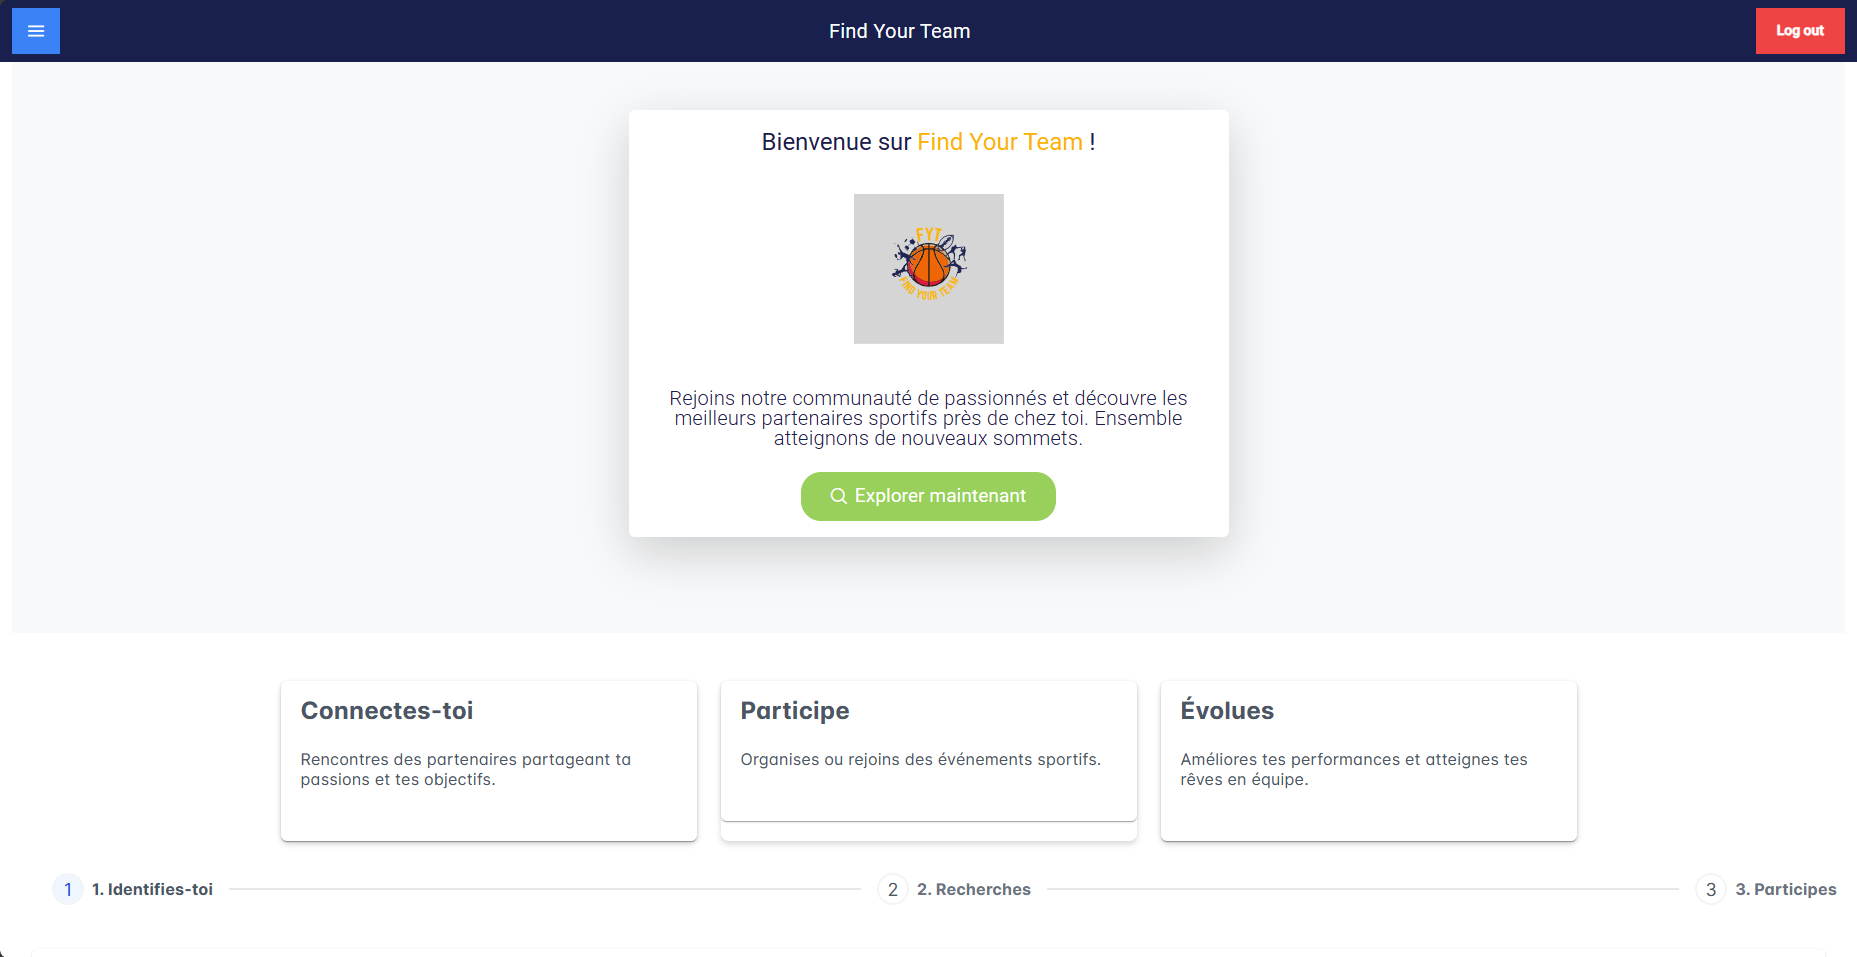
\includegraphics[width=\linewidth]{image/fytLandingPage}
        \caption{Page d'accueil lors de la connexion}
        \label{fig:fytlp}
    \end{minipage}%
    \hfill
    \begin{minipage}{.45\textwidth}
        \centering
        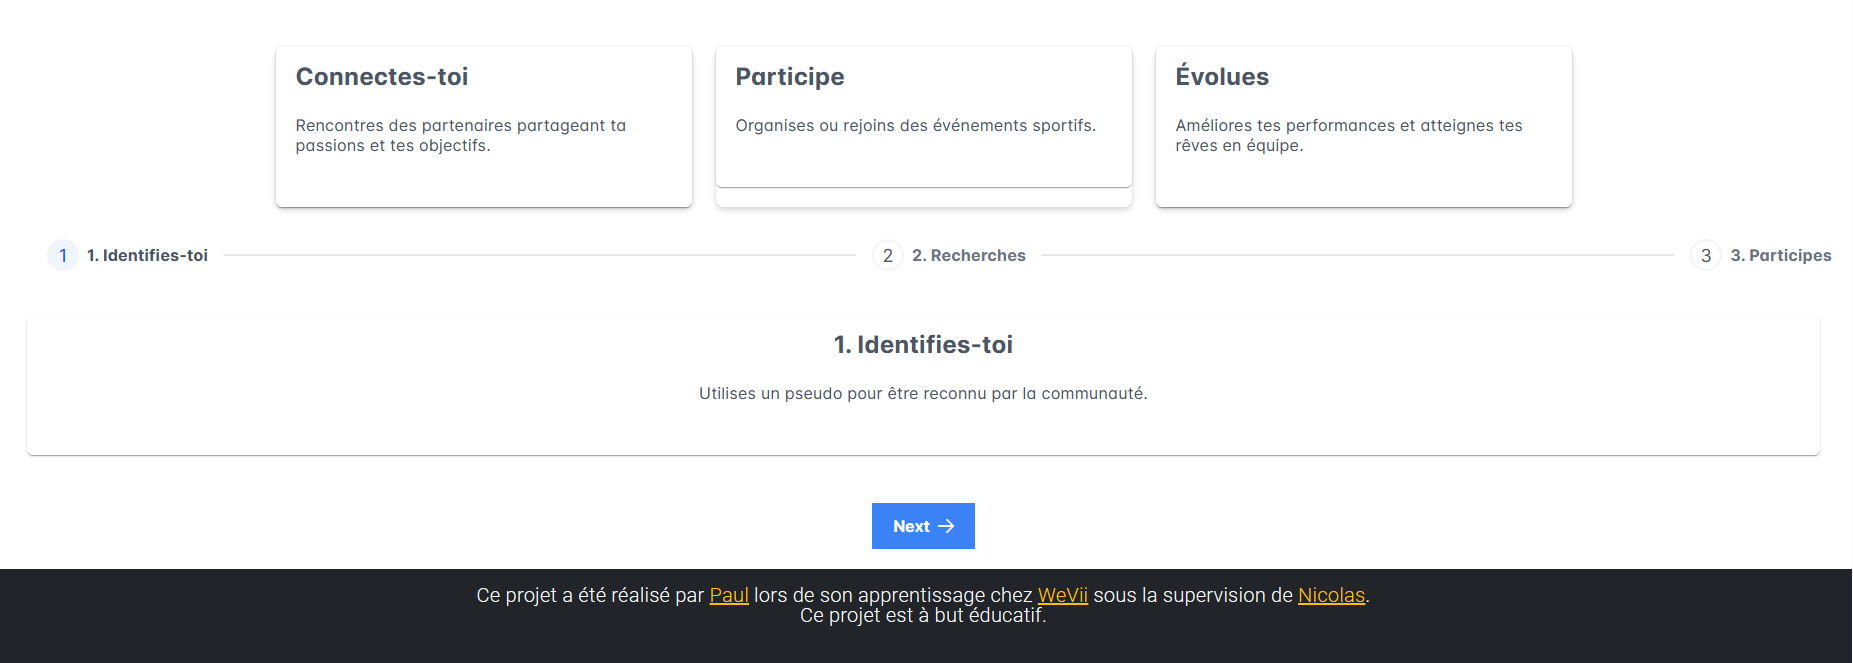
\includegraphics[width=\linewidth]{image/fytLandingPageFooter}
        \caption{Partie basse de la page d'accueil}
        \label{fig:fytlpfooter}
    \end{minipage}
\end{figure}

Les utilisateurs voulaient également un système d'authentification. Plutôt que de créer le système moi-même, j'ai utilisé Auth0, un service d'authentification facile à intégrer.
\begin{figure}[H]
    \centering
    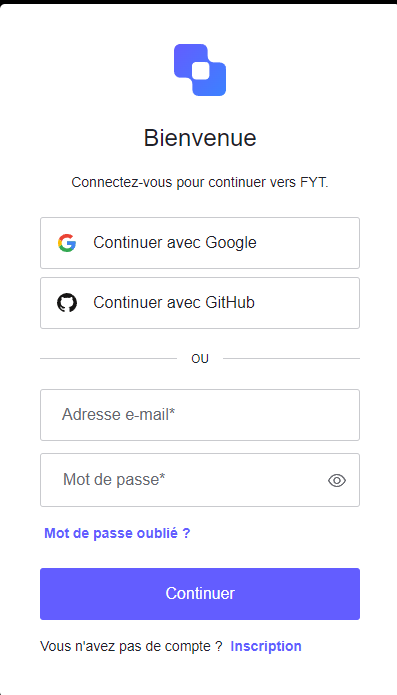
\includegraphics[width=0.35\textwidth]{image/fytAuth}
    \caption{Authentification avec Auth0}
    \label{fig:fytAuth}
\end{figure}

J'ai dû corriger des erreurs d'interface utilisateur, notamment la synchronisation entre l'ajout d'un élément et son affichage sur la carte.
Nous avions des cours sur la qualité du développement, où nous avons appris comment rendre le code plus facile à maintenir, avec des principes comme SOLID et les design patterns.
Cela m'a poussé à refactoriser le code pour le rendre plus clair et fonctionnel, par exemple en séparant le formulaire et l'affichage des événements en deux routes différentes.

\section{Déploiement et Automatisation}

Pour le déploiement, j'ai utilisé Google Cloud Run, qui exécute directement un conteneur.
J'ai également utilisé Google Cloud Artifact Registry pour stocker les images de conteneur, Cloud Build pour construire l'image automatiquement lors du déploiement continu, et Cloud Deploy pour tout déployer avec un fichier YAML.
\begin{figure}[H]
    \centering
    \begin{minipage}{.8\textwidth}
        \centering
        \begin{lstlisting}[language=Go, basicstyle=\ttfamily\scriptsize]
steps:
  - name: 'gcr.io/cloud-builders/git'
    args: ['ls', '-la', '.'] # test

  # install node package
  - name: 'node'
    entrypoint: 'npm'
    args: [ 'install' ]

  # Build Node App
  - name: 'node'
    entrypoint: 'npm'
    args: [ 'run', 'build' ]

  # Docker Build
  - name: 'gcr.io/cloud-builders/docker'
    args:
      [
        'build',
        '-t',
        ImageDocker,
        '-f',
        'Dockerfile',
        '.',
      ]

  # Docker Push to Google Artifact Registry
  - name: 'gcr.io/cloud-builders/docker'
    args: ['push', ImageDocker]

  - name: 'hashicorp/terraform'
    args: ['init']
    env: ['GOOGLE_CREDENTIALS=/workspace/account.json']

  - name: 'hashicorp/terraform'
    args: ['apply', '-auto-approve']
    env: ['GOOGLE_CREDENTIALS=/workspace/account.json']

availableSecrets:
  secretManager:
    - versionName: LienVersion
      env: 'GOOGLE_CREDENTIALS'

    # Deploy to Cloud Run
- name: 'gcr.io/cloud-builders/gcloud'
  args:
    [
      'run',
      'deploy',
      'cloudrunservice',
      '--image',
      ImageDocker,
      '--region',
      'us-central1',
      '--platform',
      'managed',
    ]
        \end{lstlisting}
        \caption{Exemple de code du fichier cloudbuild.yaml}
    \end{minipage}
\end{figure}

Google Cloud Run fourni une URL pour le service. J'ai utilisé Cloud DNS pour rediriger vers mon service Google Run pour le frontend. Mon frontend et mon backend communiquent via une API CRUD. Pour automatiser cela, j'ai créé un service en Go qui récupère l'URL du backend.
\begin{figure}[H]
    \centering
    \begin{minipage}{.8\textwidth}
        \centering
        \begin{lstlisting}[language=Go, basicstyle=\ttfamily\scriptsize]
import (
    "context"
    "github.com/gin-contrib/cors"
    "github.com/gin-gonic/gin"
    "microservice.com/appfyt/gcp"
    "net/http"
)

func getURLByName(c *gin.Context) {
    name := c.Param("name")
    c.IndentedJSON(http.StatusOK, gcp.GetURLByName(gcp.ListServicesRequest(gcp.ConnectToGCP(context.Background()), context.Background()), name))
}

func getAllUrlAndName(c *gin.Context) {
    c.IndentedJSON(http.StatusOK, gcp.GetAllUrl(gcp.ListServicesRequest(gcp.ConnectToGCP(context.Background()), context.Background())))
}

func LauncServ() {
    r := gin.Default()
    r.Use(cors.New(cors.Config{
        AllowOrigins:     []string{"*"},
        AllowMethods:     []string{"GET", "POST", "PUT", "DELETE", "OPTIONS"},
        AllowHeaders:     []string{"Origin"},
        ExposeHeaders:    []string{"Content-Length"},
        AllowCredentials: true,
    }))

    r.GET("/service/:name", getURLByName)
    r.GET("/service", getAllUrlAndName)
    r.Run(":3000")
}
        \end{lstlisting}
        \caption{Exemple de code du Service Go pour récupérer l'URL du backend}
    \end{minipage}
\end{figure}

Pour déployer ce service, j'ai utilisé Terraform, qui permet de coder l'architecture souhaitée et de créer automatiquement l'infrastructure nécessaire.
\begin{figure}[H]
    \centering
    \begin{minipage}{.8\textwidth}
        \centering
        \begin{lstlisting}[language=Go, basicstyle=\ttfamily\scriptsize]
resource "google_cloud_run_service" "microserviceurl" {
  name     = var.serviceName
  location = var.region

  template {
    spec {
      containers {
        image = var.imageMicroserviceurl
      }
    }
  }

  autogenerate_revision_name = true
}
        \end{lstlisting}
        \caption{Exemple de code Terraform pour déployer le service Go}
    \end{minipage}
\end{figure}

\section{Conclusion}

Ce projet m’a fait découvrir de nombreuses facettes du monde de l’informatique telles que le développement, le déploiement, la gestion d’une infrastructure, la sécurité ainsi que l’automatisation.
Tout ceci m’a permis de comprendre et de me rendre compte des domaines et compétences que j’apprécie et que je souhaite améliorer.

J’aime le développement avec une préférence pour le développement BackEnd.
J’ai adoré utiliser le langage Go et je souhaite m’expertiser dans ce langage.
Le développement FrontEnd n’est pas ma partie favorite car elle demande des compétences en design que je n’ai pas et qui ne me plaisent pas particulièrement.

La sécurité est une partie obligatoire et essentielle pour chaque domaine, donc il est important de connaître les bonnes pratiques en termes de cybersécurité afin de réaliser des applications et des architectures sécurisées.
La gestion de l'infrastructure, le déploiement et l'automatisation peuvent être réalisés avec du code.
C'est une partie très intéressante, surtout combinée avec le développement backend.
Cela permet d'augmenter la productivité et d'être autonome dans la mise en production des applications.

Ce projet m'a donc confirmé que je souhaite travailler dans le domaine du DevOps, qui combine développement et opérations pour améliorer et automatiser les processus de déploiement.

\clearpage
